\chapter{基于非参数模型的类音素分割}
本章主要研究类音素分割任务,这是语音研究中的一项重要任务。类音素分割和故事分割任务有一个重要的区别,即故事分割中的故事是独立不重复的,而音素单元是重复出现的。因此,本文针对类音素分割任务的这一特殊性,建立了不同于上一章的分割模型。

\section{类音素分割任务分析}
在故事分割任务中,使用了ASR的结果进行分割,但是分割效果与识别率有很大的关系,如果识别错误率较高,对后续的分割任务影响较大。如果考虑直接从音频特征寻找相似的语义单元,这样便能避免识别错误率的问题~\footnote{虽然音频层面的相似单元避免了识别错误,但是也丢失语音识别中的文本语义,使得不同语义的序列被混淆为统一模式,目前基于这一思路的方法仍在研究中。}
。一般的做法是可将任务分为词级的任务和子词级的任务进行考虑。

词级的任务是寻找语音序列中重复出现的一些具有语义的模式,类似于识别结果中的单词。子词级任务可以看做是寻找最小的发音单元,作为构成更高层次的语义单元的基本单元。如果可以很好地完成子词级任务,那么对于词级的模式发现,可以在子词单元构成的数据流上利用动态时间规整(dynamic time warp,DTW)相关的算法进行确定性匹配,找到共现的模式。这样,最终的故事分割使用的特征可以是以这些模式为维度构成的频率向量,从而避免了语音识别错误率带来的问题。

这里的子词级任务,也称为声学单元分割,由于这里声学单元类似于语音学中定义的音素概念,也称为类音素分割。有些文献也称为音素分割,不过由于音素单元具有语言学的意义,可能某个音素是有多个发音构成的,或者某些音素在一般人发音时并不区分,而这里的子词级分割主要是服务于上层任务的,所以和语言学上的音素往往并不等价。

如果不考虑样本在时间上的相关性,可以直接用有限混合模型来进行聚类,或者用Dirichlet过程混合建立无限混合模型。当得到不同观察对应的聚类后,只要将连续属于同一类目的观察当做一个音素,就可以得到一组划分。然而,如果这样做,并没有充分利用到语音数据本身的特殊性,即语音数据有很强的时序性。一方面,同一个音素对应了连续多个帧,它们的特征是相似的。另一方面,音素之间的转换具有统计意义上的差别性。如果假设帧之间是条件独立的,那么就丢失了这两点先验知识。所以这里考虑用隐马尔科模型来建模帧间的时序关系,这样就可以建模音素之间的转换关系。对于音素个数未知问题,可以利用DP的性质,建立非参数模型以自适应的发现合适的个数,上述这一模型称为分层Dirichlet过程隐马尔科夫模型(hierarchical Dirichlet process hidden Markov model,HDP-HMM)~\footnote{回顾之前的DPMM模型和dd-CRP模型,前者有较好的聚类性质,后者有较好的分割性质,而隐马尔科夫模型,即具有聚类的性质,又具有分割的性质。}。

不过,无限状态隐马尔科夫模型和传统的有限状态隐马尔科夫模型相比有一个重要的区别。由于可以有无限个状态,考虑下面这种极端情况:每一帧样本都对应一个不同的状态,即模型状态数和帧数一样大,而对于所有的t,从$z_{t-1}$到$z_t$的概率都是1,其他跳转都是0,那么这一参数是参数空间中使得模型似然最大的,但这显然不是所期望的。这里对无限状态HMM加入一个状态持续变量进行约束,使得模型有一个状态自跳转的先验,从而解决这一问题。


\section{无限状态隐马尔科夫模型}
\begin{figure}
  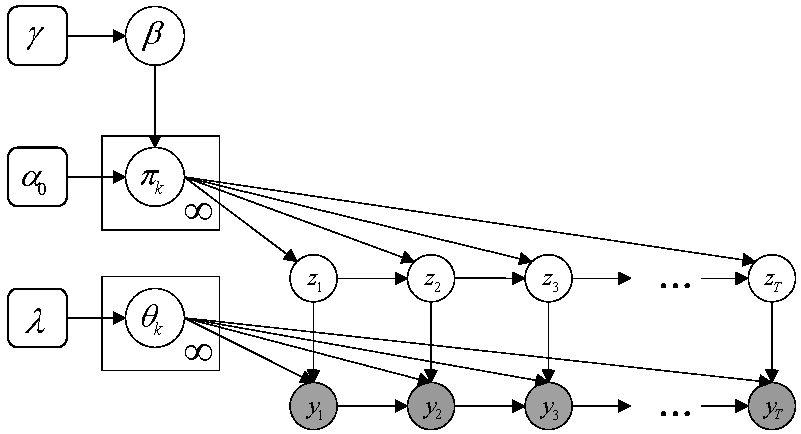
\includegraphics[width=0.8\textwidth]{ihmm_c.pdf}\\
  \caption{HDP-HMM的有向图表示}\label{fig:hdp_hmm}
  \vspace{-12pt}
\end{figure}
回顾\ref{subsec:hmm}小节中介绍的隐马尔科夫模型,其中的状态个数是固定的,$\pi_j$表示第j个状态的跳转概率,即$z_t \sim \pi_{z_{t-1}}$。回顾在\ref{sec:hdp}节介绍的HDP模型,$\pi_j$表示第j组(第j个餐馆)的参数,考虑一个含有K组数据K个共享成分(即K个餐馆K种菜品)且$K \rightarrow \infty$的HDP,如果把HMM中的K个状态看作是HDP中的K个不同的组,则可以直接将HDP中介绍的模型和推断方法用在HMM中,建立起一个含有无限个状态的HMM,参考式\eqref{eq:hdp_mix_sb},有:
\begin{equation}
\begin{split}
& {\bm \beta} \sim Gem(\gamma)\\
& {\bm \pi}_j \sim DP(\alpha_0,{\bm \beta})\\
& \theta_k \sim H\\
& z_t \sim {\bm \pi}_{z_{t-1}}\\
& x_t \sim F(\theta_{z_t}) 
\end{split}
\label{eq:hdp_hmm_sb}
\end{equation}
这一模型称之为基于HDP的无限状态HMM(HDP-HMM)(图\ref{fig:hdp_hmm})。

\section{HDP-HMM的推断方法}
回顾之前介绍的直接赋值采样方法,将${\bm \pi}$和${\bm \theta}$积分掉,并引入一个辅助变量${\bm m}$,后来证明了${\bm m}$正是CRF中的桌子数。和HDP一样,这里需要采样的变量仍然是${\bm z}$,${\bm \beta}$和${\bm m}$,采样方法几乎完全一样,唯一的区别在对${\bm z}$的采样。

在HDP中采样,当观察到${\bm \beta}$时,$z_{ji}$只跟$j$中的$z$相关,和其他的$z$是条件独立的。而此时,当观察到${\bm \beta}$,虽然不同的$j$中的$z$被${\bm \beta}$阻塞了,但是由于z之间存在连接,所以情况发生了变化。此时当观察到${\bm \beta}$,$z_{t-1}$,$z_{t+1}$时,$z_t$和其他的$z$是条件独立的,即$p(z_t = k|{\bm z}^{-t},\ beta,\alpha_0) = p(z_t = k|z_{t-1},z_{t+1},\beta,\alpha_0)$。其采样公式为:
\begin{equation}\vspace{-2pt}
\label{eq:ihmm_piror_z}
p(z_t = k|{\bm z}^{-t},\beta,\alpha_0)\!\propto\!\left\{
\begin{array}{ll}
(\alpha_0\beta_{k} + n_{z_{t-1}k}^{-t}) (\frac{\alpha_0\beta_{z_{t+1}} + n_{kz_{t+1}}^{-t} + \delta(z_{t-1},k)\delta(z_{t+1},k)}{\alpha_0 + n_k^{-t} + \delta(z_{t-1},k)} &  k \in 1,...,K \\
\alpha_0\beta_{\~{k}}\beta_{z_{t+1}} \!\! & k = \~{k} \\
\end{array}
\right.\vspace{-2pt}
\end{equation}

\section{模型的改进}
\begin{figure}
  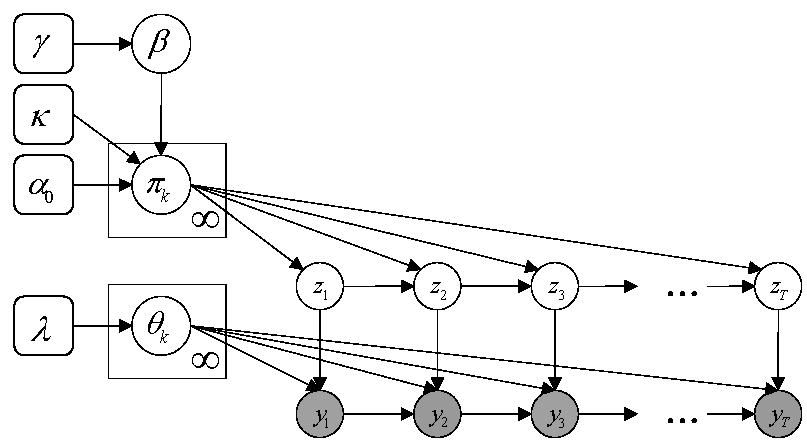
\includegraphics[width=0.8\textwidth]{sticky_ihmm_c.pdf}\\
  \caption{sticky-HDP-HMM的有向图表示}\label{fig:sticky_hdp_hmm}
  \vspace{-12pt}
\end{figure}
简单的将HMM用HDP先验扩展为一个无限状态模型存在着一个严重的问题。由于状态个数不受限制,用多个状态来表示单状态可能会有更大的似然,这是一种过拟合的情况。因为状态一般具有持续性,考虑为模型增加一个倾向于自跳转的先验知识进行规整,将式\eqref{eq:hdp_hmm_sb}中${\bm \pi}$的分布变为:
\begin{equation}
{\bm \pi}_j \sim DP(\alpha_0 + \kappa,\frac{\alpha_0{\bm \beta} + \kappa \delta_j}{\alpha_0 + \kappa})
\end{equation}
这里为自跳转的概率增加了一个大小为$\kappa$的量,得到的新模型称为sticky-HDP-HMM\cite{fox2008hdp}。其有向图表示见图\ref{fig:sticky_hdp_hmm}。

这里使用一种类似于连锁中国餐馆过程的表述来帮助理解这一模型。假设每个餐馆都有一个特色菜,第j个餐馆的特色菜就是第j道菜,注意第j道菜并不是j餐馆特有的,其他餐馆也有这道菜,但是味道要略差一些。另外,顾客的血缘关系会影响到他们的就餐习惯,若父母吃的是第j道菜,则孩子会去第j个餐馆(第j道菜是其特色菜)用餐,且更倾向于选择吃第j道菜。

将$z_t$看做父母,将$z_{t+1}$看做孩子。若$z_t = j$,则$z_{t+1}$会进入第j个餐厅,再根据$\pi_j$选择菜。

\subsection{Sticky-HDP-HMM的采样}

参考式\eqref{eq:component_num_dis},在sticky-HDP-HMM中,$\alpha_0\beta_k$变成了$\alpha_0\beta_k + \kappa \delta_{(j,k)}$,从而对${\bm m}$的采样公式为:
\begin{equation}
p(m_{jk} = m|n_{jk},\alpha_0,{\bm \beta},\kappa) = s(n_{jk},m)(\alpha_0\beta_k+ \kappa \delta_{(j,k)})^m\frac{\Gamma(\alpha_0\beta_k + \kappa \delta_{(j,k)})}{\Gamma(\alpha_0\beta_k+ \kappa \delta_{(j,k)} + n_{jk})} 
\end{equation}

考虑第$j$个餐馆第$t$个桌子上的菜,因为引入了$\kappa$,其分布变为:
\begin{equation}
k_{jt} \sim \frac{\alpha_0{\bm \beta} + \kappa \delta_j}{\alpha_0 + \kappa}\label{eq:sticky_k}
\end{equation}
辅助变量${\bm m}$和${\bm k}$有关,即$m_jk = \sum_{t=1}^{T_j}{\delta(k,k_jt)}$。Antoniak定理正是通过${\bm k}$,建立了${\bm m}$和${\bm \beta}$之间的关系,然而此时${\bm k}$的分布并不是${\bm k} \sim {\beta}$,而是式\eqref{eq:sticky_k},所以不能直接用此时${\bm k}$对应的${\bm m}$来采样${\bm \beta}$。这里引入辅助变量$\bar{k}_{jt}$和$w_{jt}$来表示$k_{jt}$:
\begin{equation}
\begin{split}
& \bar{k}_{jt}  \sim {\bm \beta}\\
& w_{jt} \sim Ber(\frac{\kappa}{\alpha_0+\kappa})\\
& k_{jt}\!\propto\!\left\{
\begin{array}{ll}
\bar{k}_{jt} & w_{jt} = 0\\
j  & w_{jt} = 1\\
\end{array}
\right.\vspace{-2pt}
\end{split}
\label{hdp_inf_aux_w}
\end{equation}
$\bar{k}_{jt}$是服从参数为${\bm \beta}$的离散分布的,所以只要求出$\bar{k}_{jt}$对应的$\bar{\bm m}$,就可以利用$\bar{\bm m}$来采样${\bm \beta}$。

$\bar{\bm m}$和${\bm m}$存在如下关系:
\begin{equation}\vspace{-2pt}
\bar{m}_{jk}\!=\!\left\{
\begin{array}{lll}
m_{jk} & k \neq j\\
m_{jj} - \sum_{t = 1}^{m_{jj}}w_{jt} & k=j\\
\end{array}
\right.\vspace{-2pt}
\end{equation}

根据上式中的关系,只要采样出$w_{jt}$,就可从${\bm m}$求得$\bar{\bm m}$,进而可以采样出${\bm \beta}$。若$k_{jt} \neq j $,则$\bar{m}_{jk} = m_{jk}$,所以只需要计算$k_{jt} = j $时的$w_{jt}$。由式\eqref{hdp_inf_aux_w},根据贝叶斯公式,得到$w_{jt}$的后验概率:
\begin{equation}\vspace{-2pt}
p(w_{jt}|k_{jt} = j,\beta,\kappa,\alpha_0)\!\propto\!\left\{
\begin{array}{lll}
\beta_j(\frac{\alpha_0}{\alpha_0+\kappa}) & w_{jt} = 0\\
\frac{\kappa}{\alpha_0+\kappa}  & w_{jt} = 1\\
\end{array}
\right.\vspace{-2pt}
\end{equation}


\section{采样方法的改进}

对于样本中两段时间上分隔同一音素单元,模型很可能先将其对应到两个不同状态,然后随着学习过程再逐渐混合为同一个状态,这一过程的速度称为混合率。直接赋值采样按照坐标轴逐个更新,混合速率较慢。这里考虑利用模型的马尔科夫性,对状态序列进行block采样。仿照隐马尔科夫模型的前向后向算法,可以进行有效的block采样,但是为了利用这一方法,必须要确定${\bm \theta}$和${\bm \pi}$的值,即也需要对这两个变量进行采样,而不是像之前那样将其积分掉。

由于模型中的状态数不确定,有限HMM的前向后向算法不能适用,所以这里考虑对GEM的一种估计,用一个L个分量的Dirichlet分布来估计DP,称为DP的自由度L的弱极限估计:
\begin{equation}
{GEM}_L(\alpha) = Dir(\frac{\alpha_0}{L},...,\frac{\alpha_0}{L}) \label{eq:L_weak_limit_approx}
\end{equation}
其中L是一个大于期望状态数的值,这种估计形式,会学到一个状态数随数据变化,以L为上界的模型。

根据式\eqref{eq:L_weak_limit_approx}这一估计形式,有:
\begin{equation}
\begin{split}
& \beta \sim Dir(\frac{\gamma}{L},...,\frac{\gamma}{L}) \\
& \pi_j \sim Dir(\alpha_0\beta_1,...,\alpha_0\beta_j + \kappa,...,\alpha_0\beta_L) 
\end{split}
\end{equation}

可以根据其后验分布进行采样:
\begin{equation}
\begin{split}
& {\beta|{\bm z},\bar{\bm {m}}} \sim Dir(\frac{\gamma}{L} + {\bar{m}}_{.1},...,\frac{\gamma}{L} + {\bar{m}}_{.L}) \\
& {\pi_j|{\bm z},\beta} \sim Dir(\alpha_0 \beta_1 + n_{j1},...,\alpha_0 \beta_j + \kappa + n_{jj},...,\alpha_0 \beta_L + n_{jL}) 
\end{split}
\end{equation}

对于${\theta}$的采样也很简单,只要根据先验和似然计算出后验即可:
\begin{equation}
\theta_j \sim p(\theta|\{y_t|z_t = j,\lambda\})
\end{equation}

这里对$z_{1:T}$进行联合采样,根据模型的马尔科夫结构,可将$z_{1:T}$的联合后验分布分解成因子相乘的形式:
\begin{equation}
\begin{aligned}
p(z_{1:T}|y_{1:T},{\bm \pi},{\bm \theta}) &=  p(z_T|z_{T-1},y_{1:T},{\bm \pi},{\bm \theta})p(z_{T-1}|z_{T-2},y_{1:T},{\bm \pi},{\bm \theta})\\
											&...p(z_2|z_{1},y_{1:T},{\bm \pi},{\bm \theta})p(z_1|y_{1:T},{\bm \pi},{\bm \theta})
\end{aligned}
\end{equation}

这样进行分解后,可先从$p(z_1|y_{1:T},{\bm \pi},{\bm \theta})$中采样出$z_1$,然后根据$z_1$的取值从$p(z_2|z_1,y_{1:T},{\bm \pi},{\bm \beta},{\bm \theta})$中采样出$z_2$,以此类推,采样出整个$z_{1:T}$。$z_t$的条件分布可以写成:
\begin{equation}
p(z_t|y_{1:T},{\bm \pi},{\bm \theta}) \propto p(z_t)p(y_t|\theta_{z_t})\sum_{z_{t+1:T}}{\prod_{t^\prime = t+1}^{T}{p(z_{t^\prime}|\pi_{z_{t^\prime-1}})p(y_{t^\prime}|\theta_{z_{t^\prime }})}}
\end{equation}

如果令$m_{t,t-1}(z_{t-1}) = \sum_{z_{t:T}}{\prod_{t^\prime = t}^{T}{p(z_{t^\prime}|\pi_{z_{t^\prime-1}})p(y_{t^\prime}|\theta_{z_{t^\prime }})}}$,则有:
\begin{equation}
p(z_t|y_{1:T},{\bm \pi},{\bm \theta}) \propto p(z_t)p(y_t|\theta_{z_t})m_{t+1,t}(z_{t})
\end{equation}

根据$m_{t,t-1}(z_{t-1})$的定义,可以得到一个$m_{t,t-1}(z_{t-1})$和$m_{t+1,t}(z_{t})$间的递推关系式:
\begin{equation}
\begin{aligned}
m_{t,t-1}(z_{t-1}) &= \sum_{z_{t:T}}{\prod_{t^\prime = t}^{T}{p(z_{t^\prime}|\pi_{z_{t^\prime-1}})p(y_{t^\prime}|\theta_{z_{t^\prime }})}} \\
   					& = \sum_{z_{t}}{p(z_{t}|\pi_{z_{t-1}})p(y_{t}|\theta_{z_{t}})  \sum_{z_{t+1:T}}{\prod_{t^\prime = t+1}^{T}{p(z_{t^\prime}|\pi_{z_{t^\prime-1}})p(y_{t^\prime}|\theta_{z_{t^\prime }})}}} \\
   					& = \sum_{z_{t}}{p(z_{t}|\pi_{z_{t-1}})p(y_{t}|\theta_{z_{t}}) m_{t+1,t}(z_{t}) }
\end{aligned}
\end{equation}
其中$m_{T+1,T}(z_{T}) = 1$,这样,只需要从马尔科夫链的尾部向头部递推的计算出$m_{t,t-1}(z_{t-1})$,然后在从头部向尾部依次采样各个$z_t$。这里称$m_{t,t-1}(z_{t-1})$为从$z_t$到$z_{t-1}$传播的后向消息。很容易证明,该方法是置信传播算法的一个特例。

\section{实验结果与分析}
\begin{figure}
\centering 
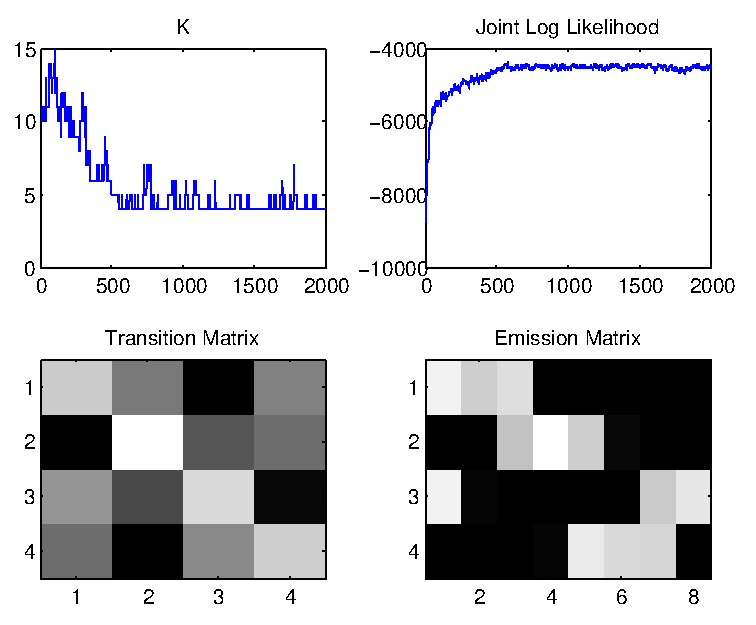
\includegraphics[width=0.7\textwidth]{gen_2000.pdf} 
\vspace{-4pt}
  \caption{2000个样本点的人工数据实验结果} \label{fig:gendata_2000}
  \vspace{-8pt}
\end{figure}
本文首先在人工生成的数据上验证算法的有效性,然后将其应用到类音素分割任务中。
\subsection{仿真实验}

仿真实验中,按照如下的模型生成含有4个隐状态、发射概率是8维的离散分布的序列数据:
\begin{equation}
A={\begin{pmatrix}
0.5&0.3&0.2&0.0\\
0.0&0.5&0.3&0.2\\
0.2&0.0&0.5&0.3\\
0.3&0.2&0.0&0.5
\end{pmatrix}}
E={\begin{pmatrix}
\frac{1}{3}&\frac{1}{3}&\frac{1}{3}&0&0&0&0&0\\
0&0&\frac{1}{3}&\frac{1}{3}&\frac{1}{3}&0&0&0\\
0&0&0&0&\frac{1}{3}&\frac{1}{3}&\frac{1}{3}&0\\
\frac{1}{3}&0&0&0&0&0&\frac{1}{3}&\frac{1}{3}
\end{pmatrix}}
\end{equation}
其中$A$是状态跳转概率矩阵,$E$中第i行对应第i个状态的离散发射概率。

利用HDP-HMM对数据进行建模和推断,对于500个样本点的数据,迭代2000次,结果如图\ref{fig:gendata_2000}。可以看出,随着算法的迭代进行,模型学习到的状态个数(K)逐渐接近真实个数,最终可以收敛到真实的状态个数。在状态转移概率和发射概率的结果图中,白色代表了1,黑色代表了0,其他颜色根据灰度值代表了0到1之间的值。可以看出,模型可以有效地推断出这两组参数。因为数据太少的缘故,得到结果和的真实的参数存在一些偏差,4状态对应了16种跳转情况,生成的500的采样点相对于这么复杂的过程,其统计性还不够。如果生成更多的数据,进行实验,则可以得到更好的结果。如图\ref{fig:gendata_5000},这是生成5000个观察样本的实验结,可见由于数据量增多,统计量更加充分,得到结果和的真实的参数之间的误差更小。
\begin{figure}
\centering 
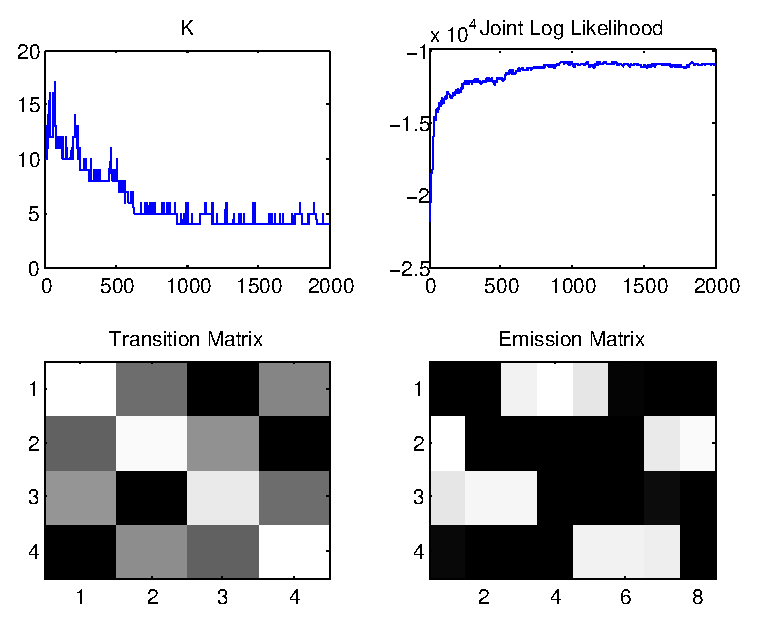
\includegraphics[width=0.7\textwidth]{gen_5000.pdf} 
\vspace{-4pt}
  \caption{5000个样本点的人工数据实验结果。可以看出,由于数据量增多,统计意义更加充分,此时的结果和真实的参数更加接近。} \label{fig:gendata_5000}
  \vspace{-8pt}
\end{figure}

\subsection{类音素分割实验结果}
实验使用TIMIT\cite{Garofolo:93:TIMIT}数据库中的语料,该数据库包含多个说话人的语音信息,每个说话人录制了多句话。语料文件命名为people-sentence。type,其中,people是不同说话人的标识,sentence是不同语句的标识\footnote{其中所有说话人都录制了SA1和SA2的语句。},type代表相应的文件类型,包括音频源文件,音素抄本,语句抄本等。其中的抄本的标注均为人工标注。本实验选用其中500句话作为实验数据。

该语料的采样频率为16K,即每秒采样16000个点。帧长25ms,帧移10ms,帧间重叠为15ms。对于每一帧数据,本实验提取13维的MFCC特征作为样本点。
\subparagraph{分割分析}
实验对本文中的方法与其他几种最新的方法进行比较,结果见表\ref{table:p_sg_result}。其中第一行是Dusan提出的一种无监督分割方法\cite{dusan2006relation},这一方法也没有假定分段的个数。第二行是Qiao提出的一种半监督的方法\cite{qiao2008unsupervised}。相比于第一行的无监督方法,本文方法的结果在各项指标上均有很大的提高,精确度、召回率和F1值分别提高了5\%、7.2\%和5.9\%。作为无监督的方法,HDP-HMM和半监督方法\cite{qiao2008unsupervised}的F1值非常接近.另外,本文的方法具有较好的召回率,这说明本文的方法在真实边界位置匹配的更好。

\begin{table}
\vspace{4pt}
\begin{center}\small
\begin{tabular}{|l|l|l|l|}
\hline \bf 方法 & \bf 正确率 & \bf 召回率 & \bf F1 \\ \hline
Dusan\cite{dusan2006relation} & 0.668 &0.752 &  0.708 \\ \hline
Qiao\cite{qiao2008unsupervised} &  0.769 & 0.775 & 0.769 \\ \hline
HDP-HMM &  0.718 & 0.824 & 0.767 \\ \hline
\end{tabular}
\end{center}
\vspace{-8pt}
\caption{分割实验结果}\label{table:p_sg_result}
\vspace{-4pt}
\end{table}
%我们对分割结果进行更细致的观察分析,取两个不同说话人SA1中各个单词对应的结果。见表xxx。
%(这里需再制一张表,包括两个不同说话人SA1中的各个单词对应的聚类结果。)

\begin{figure}
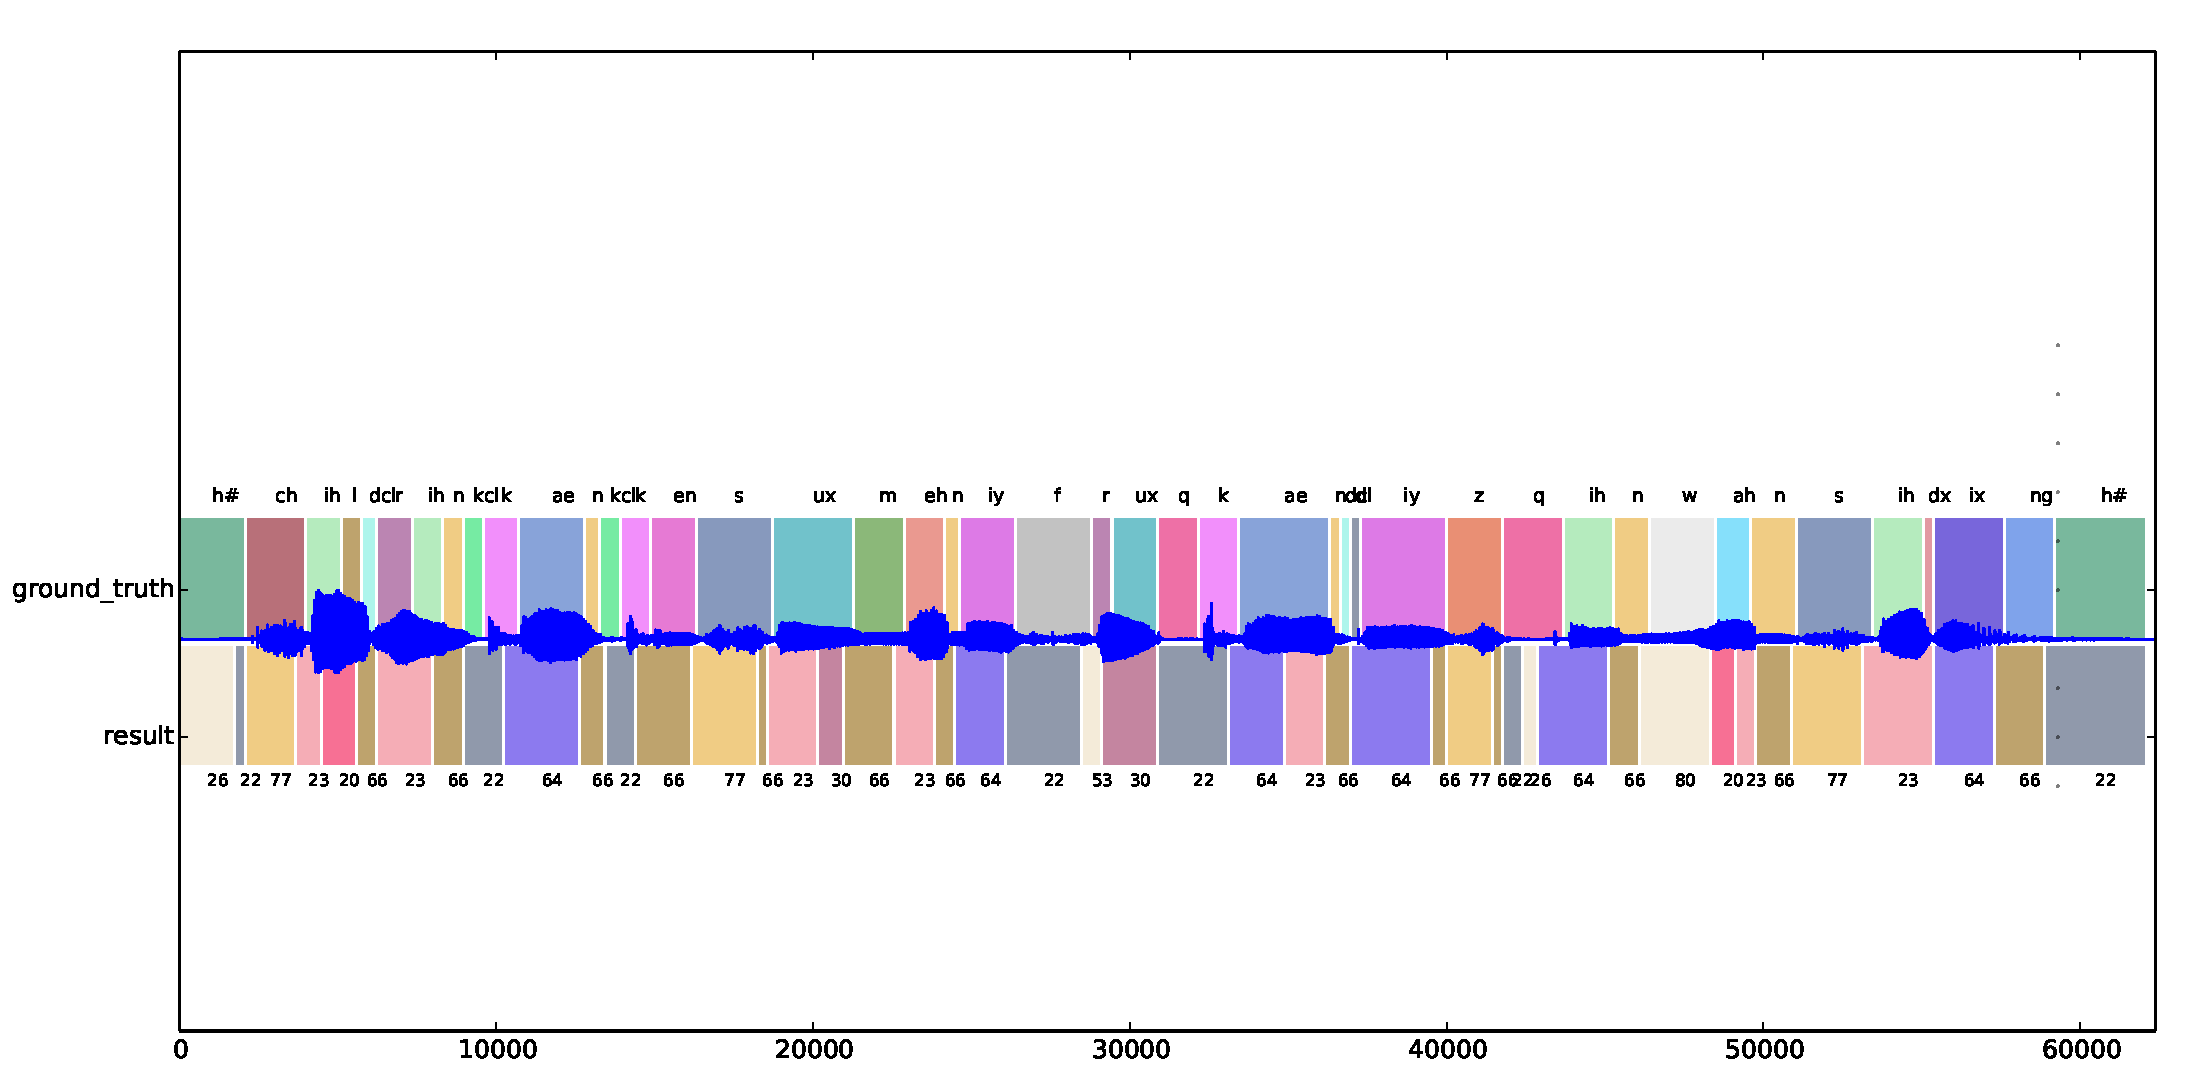
\includegraphics[width=\textwidth]{SX398_analysis.pdf} 
\vspace{-4pt}
  \caption{语料FKAA0-SX398上的实验结果,其中横坐标以采样点为单位。这段话的抄本为“Children can consume many fruit candies in one sitting”。语料的采样频率为16K,包含62362个采样点。由于mfcc特征文件丢弃了最后的一部分静音段,所以图中的标注和实验结果序列均比语音序列短一些。} \label{fig:SX398_analysis}
  \vspace{-8pt}
\end{figure}

\subparagraph{聚类分析}
\begin{figure}
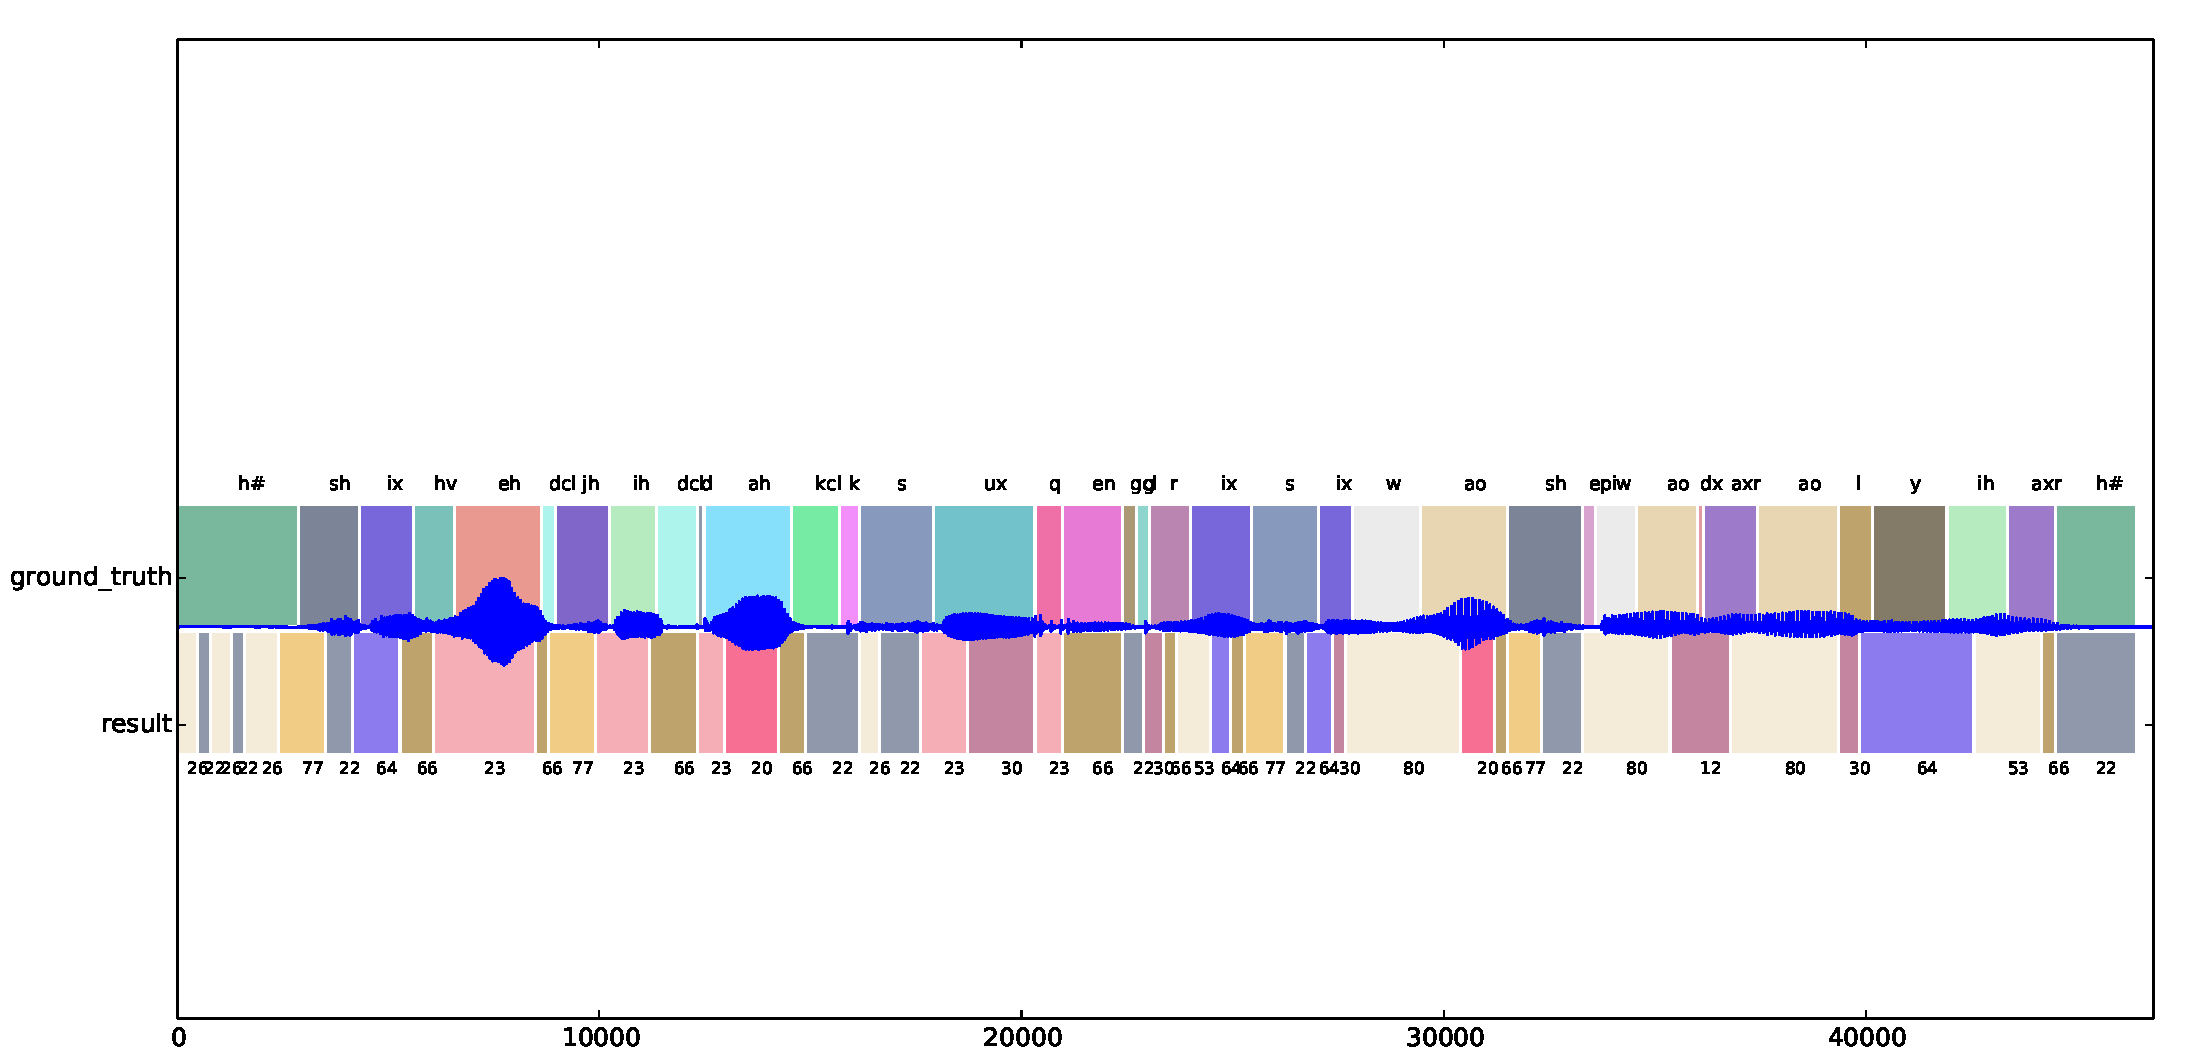
\includegraphics[width=\textwidth]{SA1_analysis.pdf} 
\vspace{-4pt}
  \caption{语料FCJF0-SA1上的实验结果。这段话的抄本为 “She had your dark suit in greasy wash water all year”。
.} \label{fig:SA1_analysis}
  \vspace{-8pt}
\end{figure}

HDP-HMM模型在建模时就考虑到了数据的聚类特征,因此,除了对单元分割的结果进行评估,本文也对其聚类的效果进行分析,如图\ref{fig:SX398_analysis},展示了语料FKAA0-SX298上的实验结果,图中底端是分割聚类的结果,中间是音频原始信号,上端是真实的音素标注。上端的白线表示真实音素边界,相同颜色块对应同一个的音素,下端的白线表示结果中的边界,相同颜色块对应同一个的聚类。
对于一些音素,如ix,iy和ih,er和axr,无论是人耳的听音,还是从音频信号上观察都非常相近,算法将这些相似的音素合并成一类,所以聚类的个数会比真实音素个数少一些。本文分析了多组语料上的结果(图\ref{fig:SA1_analysis}展示了语料FCJF0-SA1上的结果),直观的研究聚类状态和真实音素之间的关系,表\ref{table:c_p_relation}给出了一些相关性明显的聚类,可以看出,和i(音一)相近的发音ix,iy,ih都被聚成到64类,s,z等音被聚到77类,en,n,ng等鼻音被聚到66类。几乎所有的语料,h\#(静音段)都被聚为22类,而一些清辅音如k,f,q也被分到22类,这是因为这些清辅音能量较小,不容易区分开。

\begin{table}
\vspace{4pt}
\begin{center}\small
\begin{tabular}{|l|l|}
\hline \bf 聚类类目 & \bf 对应的音素 \\ \hline
64 &  iy,ih,ix \\ \hline
77 &  s,z \\ \hline
66 &  en,n,ng \\ \hline
22 &  h\#,k,f,q \\ \hline
80 &  ao,aa \\ \hline
\end{tabular}
\end{center}
\vspace{-8pt}
\caption{实验的一些聚类结果,可以看出,HDP-HMM找到的类目相较于真实音素个数少一些,不过却具有很明显的物理意义,即同一族的音素被聚到了一类}
\vspace{-4pt}
\end{table}\label{table:c_p_relation}